%%%%%%%%%%%%%%%%%%%%%%%%%%%%%%%%%%%%%%%%%
% Masters/Doctoral Thesis 
% LaTeX Template
% Version 1.43 (17/5/14)
%
% This template has been downloaded from:
% http://www.LaTeXTemplates.com

% Original authors:
% Steven Gunn 
% http://users.ecs.soton.ac.uk/srg/softwaretools/document/templates/
% and
% Sunil Patel
% http://www.sunilpatel.co.uk/thesis-template/
%
% License:
% CC BY-NC-SA 3.0 (http://creativecommons.org/licenses/by-nc-sa/3.0/)
%
% Note:
% Make sure to edit document variables in the Thesis.cls file
%
%
% Modified and Adapted by Michael Lees 2020
%%%%%%%%%%%%%%%%%%%%%%%%%%%%%%%%%%%%%%%%%

%----------------------------------------------------------------------------------------
%	PACKAGES AND OTHER DOCUMENT CONFIGURATIONS
%----------------------------------------------------------------------------------------

\documentclass[11pt, oneside, dvipsnames]{Thesis} % The default font size and one-sided printing (no margin offsets)

\graphicspath{{Figures}} % Specifies the directory where pictures are stored


\usepackage[square, numbers, comma, sort&compress]{natbib} % Use the natbib reference package - read up on this to edit the reference style; if you want text (e.g. Smith et al., 2012) for the in-text references (instead of numbers), remove 'numbers' 
\usepackage[ruled,vlined]{algorithm2e}
\usepackage{amsmath}
\usepackage{enumitem}
\setlist{nolistsep}
\usepackage{booktabs}

\usepackage[Sonny]{fncychap}
\ChNameUpperCase
\ChNumVar{\fontsize{30}{35}\usefont{OT1}{ptm}{m}{n}\selectfont}
\ChTitleVar{\Large\sc}

\usepackage{titlesec}
\DeclareMathOperator*{\argmin}{arg\,min}
\DeclareMathOperator*{\argmax}{arg\,max}
\title{\ttitle} % Defines the thesis title - don't touch this

\begin{document}

\frontmatter % Use roman page numbering style (i, ii, iii, iv...) for the pre-content pages
\setstretch{1.3} % Line spacing of 1.3

% Define the page headers using the FancyHdr package and set up for one-sided printing
\fancyhead{} % Clears all page headers and footers
\rhead{\thepage} % Sets the right side header to show the page number
\lhead{} % Clears the left side page header

\pagestyle{fancy} % Finally, use the "fancy" page style to implement the FancyHdr headers

\newcommand{\HRule}{\rule{\linewidth}{0.5mm}} % New command to make the lines in the title page


% Command for Social choice
\newcommand{\alternatives}{X}
\newcommand{\voters}{N}
\newcommand{\pref}{\succ}
\newcommand{\prefmaj}{\succ_{\text{maj}}}
\newcommand{\domain}[1]{\mathcal{D}_{\text{#1}}}
\newcommand{\votingrule}[1]{f_{\text{#1}}}
\newcommand{\orderalt}{\triangleleft}

% PDF meta-data
\hypersetup{pdftitle=\ttitle}
\hypersetup{pdfsubject=\subjectname}
\hypersetup{pdfauthor=\authornames}
\hypersetup{pdfkeywords=\keywordnames}

%----------------------------------------------------------------------------------------
%	TITLE PAGE
%----------------------------------------------------------------------------------------

\begingroup
\hypersetup{
	urlcolor=black
}
\begin{titlepage}
\begin{center}

\textsc{\LARGE \univname}\\[1.5cm] % University name
\textsc{\Large Masters Thesis}\\[0.5cm] % Thesis type

\HRule \\[0.4cm] % Horizontal line
{\huge \bfseries \ttitle}\\[0.4cm] % Thesis title
\HRule \\[1.5cm] % Horizontal line
 
\begin{minipage}{0.4\textwidth}
\begin{flushleft} \large
\emph{Author:}\\
\href{http://amirsahrani.com}{\authornames} % Author name - remove the \href bracket to remove the link
\end{flushleft}
\end{minipage}
\begin{minipage}{0.4\textwidth}
\begin{flushright} \large
\emph{Examiner:} \\
{\exname}\\
\emph{Supervisor:} \\
{\supname}\\
\emph{Assessor:} \\
{\assessorname}
\end{flushright}
\end{minipage}\\[1cm]
 
\large \textit{A thesis submitted in partial fulfilment of the requirements\\ for the degree of \degreename}\\[0.3cm] % University requirement text
\textit{in the}\\[0.4cm]
\groupname\\\deptname\\[2cm] % Research group name and department name
 
{\large \today}\\[2cm] % Date
% 
\includegraphics[width=0.6\textwidth]{clslogo.png} % Include Computational Science Logo
 
\vfill
\end{center}

\end{titlepage}
\endgroup

%----------------------------------------------------------------------------------------
%	DECLARATION PAGE
%	Your institution may give you a different text to place here
%----------------------------------------------------------------------------------------

\Declaration{

\addtocontents{toc}{\vspace{1em}} % Add a gap in the Contents, for aesthetics

I, \authornames, declare that this thesis, entitled `\ttitle' and the work presented in it are my own. I confirm that:

\begin{itemize} 
\item[\tiny{$\square$}] This work was done wholly or mainly while in candidature for a research degree at the University of Amsterdam.
\item[\tiny{$\square$}] Where any part of this thesis has previously been submitted for a degree or any other qualification at this University or any other institution, this has been clearly stated.
\item[\tiny{$\square$}] Where I have consulted the published work of others, this is always clearly attributed.
\item[\tiny{$\square$}] Where I have quoted from the work of others, the source is always given. With the exception of such quotations, this thesis is entirely my own work.
\item[\tiny{$\square$}] I have acknowledged all main sources of help.
\item[\tiny{$\square$}] Where the thesis is based on work done by myself jointly with others, I have made clear exactly what was done by others and what I have contributed myself.
\end{itemize}


Signed: 

\vspace{1em}


\includegraphics[width=3cm]{Figures/yoursignature.pdf} \par
 
Date: \today
}

\clearpage % Start a new page

%----------------------------------------------------------------------------------------
%	QUOTATION PAGE
%----------------------------------------------------------------------------------------

\pagestyle{empty} % No headers or footers for the following pages

\null\vfill % Add some space to move the quote down the page a bit

\textit{``The majority, standing in for the people, wills everything and therefore wills nothing"}

\begin{flushright}
	Joshua Cohen
\end{flushright}

\vfill\vfill\vfill\vfill\vfill\vfill\null % Add some space at the bottom to position the quote just right

\clearpage % Start a new page

%----------------------------------------------------------------------------------------
%	ABSTRACT PAGE
%----------------------------------------------------------------------------------------

\addtotoc{Abstract} % Add the "Abstract" page entry to the Contents

\abstract{\addtocontents{toc}{\vspace{1em}} % Add a gap in the Contents, for aesthetics

Include your abstract here 
Abstracts must include sufficient information for reviewers to judge the nature and significance
of the topic, the adequacy of the investigative strategy, the nature of the results, and the
conclusions. The abstract should summarize the substantive results of the work and not merely
list topics to be discussed. 

Length 200-400 words.
}

\clearpage % Start a new page

%----------------------------------------------------------------------------------------
%	ACKNOWLEDGEMENTS
%----------------------------------------------------------------------------------------

\setstretch{1.3} % Reset the line-spacing to 1.3 for body text (if it has changed)

\acknowledgements{\addtocontents{toc}{\vspace{1em}} % Add a gap in the Contents, for aesthetics

Thank the people that have helped, supervisors family etc.

}
\clearpage % Start a new page

%----------------------------------------------------------------------------------------
%	LIST OF CONTENTS/FIGURES/TABLES PAGES
%----------------------------------------------------------------------------------------

\pagestyle{fancy} % The page style headers have been "empty" all this time, now use the "fancy" headers as defined before to bring them back

\lhead{\emph{Contents}} % Set the left side page header to "Contents"
\tableofcontents % Write out the Table of Contents


\lhead{\emph{List of Figures}} % Set the left side page header to "List of Figures"
\listoffigures % Write out the List of Figures

\lhead{\emph{List of Tables}} % Set the left side page header to "List of Tables"
\listoftables % Write out the List of Tables

\lhead{\emph{List of Algorithms}} % Set the left side page header to "List of Algorithms"
\addtotoc{List of Algorithms}
\listofalgorithms % Write out the List of Tables

%----------------------------------------------------------------------------------------
%	ABBREVIATIONS
%----------------------------------------------------------------------------------------

\clearpage % Start a new page

\setstretch{1.5} % Set the line spacing to 1.5, this makes the following tables easier to read

\lhead{\emph{Abbreviations}} % Set the left side page header to "Abbreviations"
\listofsymbols{ll} % Include a list of Abbreviations (a table of two columns)
{
\textbf{CSL} & \textbf{C}omputational \textbf{S}ceince \textbf{L}ab\\
\textbf{UvA} & \textbf{U}niversitiet \textbf{v}an \textbf{A}msterdam\\
%\textbf{Acronym} & \textbf{W}hat (it) \textbf{S}tands \textbf{F}or \\
}
%----------------------------------------------------------------------------------------
%	PHYSICAL CONSTANTS/OTHER DEFINITIONS
%----------------------------------------------------------------------------------------

%\lhead{\emph{Physical Constants}} % Set the left side page header to "Physical Constants"

%\listofconstants{lrcl} % Include a list of Physical Constants (a four column table)
%{
%Speed of Light & $c$ & $=$ & $2.997\ 924\ 58\times10^{8}\ \mbox{ms}^{-\mbox{s}}$ (exact)\\
%% Constant Name & Symbol & = & Constant Value (with units) \\
%}

%----------------------------------------------------------------------------------------
%	SYMBOLS
%----------------------------------------------------------------------------------------

\clearpage % Start a new page

\lhead{\emph{Symbols}} % Set the left side page header to "Symbols"

\listofnomenclature{ll} % Include a list of Symbols (a three column table)
{
$N$ & The set of all voters\\
$X$ & The set of all alternatives\\
$\pref$ & A preference relation ship\\
$\domain{ }$ & A domain of possible profiles\\
$\orderalt$ & A geometric order over candidates\\
}

%----------------------------------------------------------------------------------------
%	DEDICATION
%----------------------------------------------------------------------------------------

\setstretch{1.3} % Return the line spacing back to 1.3

\pagestyle{empty} % Page style needs to be empty for this page

\addtocontents{toc}{\vspace{2em}} % Add a gap in the Contents, for aesthetics

%----------------------------------------------------------------------------------------
%	THESIS CONTENT - CHAPTERS
%----------------------------------------------------------------------------------------

\mainmatter % Begin numeric (1,2,3...) page numbering

\pagestyle{fancy} % Return the page headers back to the "fancy" style

% Include the chapters of the thesis as separate  tex files from the Chapters folder
% Change the file names if you prefer

%This structure provides a bare bones essentials of the thesis and some indicative length
%This structure may not fit your thesis perfectly, but be sure to include these components somehow.
%It is possible to split the chapters up (E.g., 2 methods chapter, Experiment and Results as two, etc.)

% The typical length may be between 43 - 64 pages. Do not worry if you go slightly larger or smaller than this. 
% But a thesis of 20 pages, or 100 pages may suggest you've been to brief or too verobse.
%NOTE - there is not strict limit/minimum.

\newpage
\chapter{Introduction}
\label{Introduction}
\lhead{\emph{Introduction}} % Set the left side page header to "Symbols"

Many Democracies suffer from polarization and misinformation, leading to a
general dissatisfaction with the process under voting populations. As a result
of this polarization and misinformation, voters get more extreme opinion, but
also more skewed views of the other end of the spectrum. As a result any
elections not only have the difficult task of electing candidates that please
as many people as possible, they have to do this while people have different
idea's about the problems and candidates in the first place.

For democracy to function effectively, voters need a shared foundation of
understanding, what we term a ``shared reality.'' This shared reality consists
of commonly accepted facts and causal relationships that allow meaningful
debate about policy trade-offs. For example, most economists agree that raising
minimum wages typically increases costs for businesses, which may lead to
higher consumer prices. When voters share this understanding, they can engage
in productive disagreement about whether wage increases are worth the potential
price increases. However, when some voters believe wage increases lead to
increased prices while others believe these to be unrelated, an election
seemingly about purchasing power policies becomes an inaccurate measure of
people's true intentions.

Historically, people's understanding of the world came primarily from personal
networks, family, friends, and colleagues who shared similar experiences and
information sources. Increasingly, however, algorithmic curation shapes
individual worldviews. This creates a fundamental problem: because algorithms
tailor content to individual preferences, each person may encounter a unique
set of claims about how the world works, leading to fragmented understandings
of reality.

As a result of fragmented world views, what was once a clear problem can become
messy with alternate unrelated problems. As a corollary to this, during
elections people might be voting in favor of some outcome for different, and
possibly opposing reasons. For example voting for some candidate thinking they
will lower grocery prices while also increasing the minimum wage, which, in
general are opposing forces. We later formalize this notion of a ``reason''
through the concept of the \textit{Issue Dimension}
\cite{listTwoConceptsAgreement2002}, when people have a common \textit{Issue
	Dimension}, all their differences in opinion on outcomes can be explained
through these dimensions. In the case of higher wages v.s. lower prices, for
example, a difference in opinion could be explained as favoring higher wages
as general costs will rise proportionally less.

From a social choice perspective, having shared issue dimensions can be very beneficial, especially if
in the case of a singular dimension. In this special case, we
might get ``single-peaked'' preferences, . In \Cref{Literature} we explain what
this means exactly, and why it is desirable. For now, it
suffices to note that they allow for elections mechanisms which encourage
voters to be honest about their preferences. We explain what we mean exactly by
an election mechanism in \Cref{chap: preliminaries}, but intuitively it is
simply a way to pick a winner from a set of preferences.

To increase the single-peakedness of voter preferences,
\citet{listDeliberationSinglePeakednessPossibility2013} propose deliberation
as a potential solution. Building on List's \cite{listTwoConceptsAgreement2002}
concept of meta-agreement, the idea that voters must agree on which issue
dimensions matter and where candidates stand on these dimensions. List et al. argue
that deliberation can help voters develop more coherent preference structures.
This is particularly valuable for low-salience issues that receive little
public attention, where deliberation can both increase voter knowledge and
produce preference profiles closer to single-peaked

Given deliberation's potential to lead to this meta-agreement and possibly to
nicely structured preferences, we think it important to understand
deliberation more deeply.  As in-silico experiments become more important parts
of socio-political modeling, we choose a computational approach to
understanding deliberation. Specifically, we adapt the DeGroot model
\cite{degrootReachingConsensus1974} to fit deliberation on voter opinions and
candidate's positions.

To this end, in \Cref{Literature} we present relevant work on
single-peakedness, deliberation, and experiments, as well as presenting a
deliberation model by \citet{radDeliberationSinglePeakednessCoherent2021}. In
\Cref{theory} we formally define some properties of deliberation, and prove
negative results regarding ``Honesty'' during deliberation, showing
deliberation is not strategyproof under a variety of circumstances. We also
define an adaptation to the DeGroot model, as a mechanistic explanation of
deliberation through a computational model. In doing so, we find a limitation
in the applicability of  this model in the form of a negative computational
complexity result, we show NP-completeness of mapping voter opinions to trust
matrices. In \Cref{Methods} we explain the experimental setup we use to test
our model, the result of which we present in \Cref{experiment_results}.
Finally, we reflect on the results and methods in \Cref{Discussion}.

 %Set out your thesis and state your research question (5-8 pages)
\newpage
\chapter{Literature review}
\label{Literature}

\lhead{\emph{Literature Review}} % Set the left side page header to "Symbols"





\section{Condorcet Domain}
If our goal is to prevent Condorcet cycles, or in general have transitive majority relations, the best we could hope to do is to apply our domain restriction such that our domain contains all profiles $P$ such that $P$ has a (weak) Condorcet winner. We call this domain $\domain{Condorcet}$. Under this domain, let $\votingrule{Condorcet}$ be the Condorcet Rule, which picks a Condorcet winner. Then $\votingrule{Condorcet}$ is strategyproof over $\domain{Condorcet}$ \citep{elkindPreferenceRestrictionsComputational2022}.

\begin{proofc}{(\citet{elkindPreferenceRestrictionsComputational2022})}.
    Assume, for the sake of a contradiction, we have profiles $P = (\pref_1 \dots \pref_i \dots \pref_n)$ and $P' = (\pref_1 \dots \pref_{i'} \dots \pref_n)$ such that:
    \[
        \votingrule{Condorcet}(P) = a, \quad \votingrule{Condorcet}(P') = b, \quad \text{and } a \neq b
    \]
    Then under $P$ a strict majority $N' \subseteq N$ have $a \pref b$, but $i \notin N'$, thus in $P'$, $N'$ is still a majority preferring $a$ to $b$, but this is in contradiction to $b$ winning in $P'$.
\end{proofc}


Though this result is positive, $\domain{Condorcet}$ is not hereditary, this is easy to see through an example:
\begin{example}{$\domain{Condorcet}$ is not hereditary}{con-her}
    \begin{minipage}{0.25\linewidth}
        \begin{tabular}{cccc}
            \toprule
            $v_1$ & $v_2$ & $v_3$ & $v_4$ \\
            \midrule
            a     & b     & c     & a     \\
            b     & c     & a     & c     \\
            c     & a     & b     & b     \\
            \bottomrule
        \end{tabular}
    \end{minipage}
    \begin{minipage}[b]{0.70\linewidth}
        We can see that in this example, $a$ is the weak Condorcet winner, as it beats $b$ and is tied with $c$, however if we remove voter 4, we return to the original Condorcet cycle.
    \end{minipage}
\end{example}

A domain not being hereditary means that the nice properties of the domain can be unstable, as the number of voters and alternatives might not be known or could be manipulated. Instead, we might want to look at hereditary domains.

\subsection{Hereditary Domains}

\begin{definition}{Hereditary \textnormal{(\citet{elkindPreferenceRestrictionsComputational2022})}}{dom-hereditary}
    A domain restriction onto $\domain{ }$ is \textit{hereditary} if, for every profile $P \in \domain{ }$, and every profile $P'$, that can be obtained by deleting voters and alternatives from $P$, $P'$ is also in $\domain{ }$
\end{definition}


The first hereditary domain we present, will also be the main focus of this thesis. This is the domain of all single-peaked profiles.


Note that in  a voter is allowed to prefer $b$ best, and then choose $a$ or $c$ in any order. It is clear to see that if any voter or alternative is deleted, this property is satisfied.

\begin{proposition}{\textnormal{(\citet{elkindPreferenceRestrictionsComputational2022}).}}
    $\domain{SP}$ is hereditary.
\end{proposition}

\begin{proof}
    (Voter Deletion). If we remove a voter, this does not affect the other voters, thus the property is satisfied.~\checkmark

    (Alternative Deletion). Consider a voter $i$ and their single-peaked vote, if we remove some alternative $x$, this voter all alternatives which voter $i$ preferred to $x$ stay in the same position, while all other alternatives move up one rank, thus preserving the order.~\checkmark
\end{proof}

A similar notion to single-peaked profiles is that of single caved profiles, which is equivalent, but instead a voters peak representing their most preferred option, they have a valley, which represents the worst option. Single caved profile are hereditary as well, but for a voting rule on them to be strategy proof, only two possible alternatives can be chosen, the left and right most alternatives according to $\orderalt$.

Instead of ordering the alternatives, we can imagine instead ordering the voters, such that we have a leftmost and rightmost voters, and all other voters can be placed between them based on their difference. In this case, a profile is single-crossing if, for any alternative $a$, its preference relation to another any alternative $b$ flips at most once when traversing the voters in order $\orderalt$.

\begin{definition}{Single-Crossing Profiles \textnormal{(\citet{elkindPreferenceRestrictionsComputational2022})}}{single-crossing}
    A profile $P$ is single-crossing w.r.t. some ordering $\orderalt$, if for any $a,b \in X$, $\{i \in N : a \pref b\}$ and $\{i \in N: b \pref a\}$ are both intervals over $[n]$. A profile $P$ is single crossing if the votes can be permuted such that it is single crossing w.r.t. a given ordering.
\end{definition}

Similar to single-peaked profiles, the domain of single-crossing profiles, $\domain{SC}$ is also hereditary

\begin{proposition}
    $\domain{SC}$ is hereditary
\end{proposition}

\begin{proof}
    (Voter Deletion). Deleting a voter preserves the ordering between voters, as such this cannot introduce a new crossing between alternatives.~\checkmark

    (Alternative Deletion). If we remove an alternative the voters' rankings of the other alternatives does not change, thus preserving single-crossing.~\checkmark
\end{proof}

\section{The History of Deliberation and Meta-Agreement}

We have provided an overview of different domain restriction and their properties, mainly showing how they avoid Condorcet cycles. Some argue however, that Condorcet cycles are empirically rare. The next section is dedicated to explaining why this is so through examining the historical ideas around deliberation and deliberative democracy, as well as that of Meta-Agreement.

\subsection{Deliberation}
Though deliberation is intuitively familiar, namely the process of multiple people talking through a problem with the goal of coming to an agreement, compromise or solution, providing a definition that is both clear and consistent with the literature in Political Science, Philosophy and Social choice is difficult.  This intuition it leaves some of the reasons for and goals of deliberation, as state in the literature, unmentioned.


\citet{freemanDeliberativeDemocracySympathetic2000} gives an overview of deliberative democracy, in which he shares the intuitive idea that a deliberative democracy contains open discussion, open legislative deliberation and a pursuit of the common good. He also notes that there is no common agreement on the central features of a deliberative democracy, one account is that of deliberative democracy simply involving discussion among the public before voting. Another similar account is that this voting must not only be preceded by deliberation, but also general communication, all of which intended to change people's preferences. He further proceeds to give a more detailed conception of deliberative democracy, according to which a deliberative democracy is one in which political agents or their representatives

\begin{enumerate}
    \label{list:deliberative-democracy}
    \setlength\itemsep{1px}
    \item  Aim to collect, deliberate and vote
    \item  Represent their sincere and informed judgements
    \item  Vote and deliberate on measures beneficial to the common good on the citizens
    \item  Are seen and see each other as political equals
    \item  Have Constitutional right and social means enables them to participate in public life
    \item  Are individually free, such that they have their own freely determined conceptions of the good
    \item  Have diverse and disagreeing conceptions of the good
    \item  Recognize and accept their duty as democratic citizens, and do not engage in public argument on the basis of their particular moral views incompatible with public reason.
    \item  Agree reason is public, in so much as it is related to and advances common interests of citizens
    \item  Agree that their common interest lies primarily in freedom, independence and equal status as citizens.
\end{enumerate}

These features allow us to be more precise when we talk about a deliberative democracy, and in turn be more careful about what deliberation must entail. \citet{cohenDeliberationDemocraticLegimitimacy2002} further argues that deliberation is needed for democratic legitimacy. By this he means that without deliberation, a democracy is simply the will of the majority, but since majority rule is unstable, it is simply a reflection of the particular institutional constrains at the time. He further goes on to describe the \textit{ideal deliberative procedure} as follows

\begin{enumerate}
    \label{list:ideal-deliberation}
    \setlength\itemsep{1px}
    \item  Ideal deliberation is \textit{free}, participants regard themselves as only bound by the results of the deliberation, and the preconditions thereof. Participants act in accordance with the decision made through deliberation, and it being agreed on is sufficient reason to do so.
    \item  Ideal deliberation is \textit{reasoned}, parties are required to state their reasons for advancing proposals.
    \item  In ideal deliberation, parties are \textit{equal}, both formally and substantively. There are no rules that single individuals out, and existing distributions of power to no lend a party the opportunity to contribute to deliberation.
    \item  Ideal deliberation aims to arrive at \textit{consensus}, which can be rationally defended.
\end{enumerate}

\subsection{Meta-Agreement}
\label{subsection:Meta-agreement}

A goal of deliberation could be to reach consensus, which is sometimes referred to as substantive agreement, \citet{elsterMARKETFORUMThree2002} argues that this is not only the goal, but through unanimity this process completely replaces voting, thereby circumventing Arrow's impossibility theorem: ``Or rather, there would not be any need for an aggregation mechanism, since a rational discussion would tend to produce unanimous preferences.” (p. 112). Though it would be desirable to circumvent Arrow's impossibility theorem, in practice people, even after deliberation might not, indeed often do not, come to full substantive agreement. \citet{listTwoConceptsAgreement2002} instead proposed another lens through which we can analyze deliberation and the type of agreement it induces.

Under \emph{Meta-agreement} individuals do not need to agree on their most preferred outcome, instead they only need to agree on the dimensions of the problem. To contrast this with substantive agreement, under which individuals do not need to conceive of the problem in the same way, all they need is to agree on the same outcome. This means that under substantive agreement, voters can agree outcome $a \pref b$ for different reasons, while under meta-agreement, if voters disagree on $a \pref b$ it must be for the same reason.

According to \citet{listTwoConceptsAgreement2002} there are three hypotheses that need to be satisfied for deliberation to induce meta-agreement:
\begin{enumerate}
    \label{list:meta-agreement-checklist}
    \setlength\itemsep{1px}
    \item [D1] Deliberation leads people to discover a single \textit{issue}-dimension
    \item [D2] Deliberation lets people place all possible alternatives in this \textit{issue}-dimension
    \item [D3] After this deliberation, people update their preferences by picking
          a preferred outcome, and all other rankings are based on the distance to this outcome in the \textit{issue}-dimension
\end{enumerate}

All these are necessary conditions for meta-agreement, from this is it also clear to see that, given that there is exactly 1 \textit{issue}-dimension, single-peaked profile are, by definition, a direct consequence. This is the main reason meta-agreement is desirable, as it lets us circumvent the Gibbard-Satterthwaite theorem \citep{gibbardManipulationVotingSchemes1973, satterthwaiteStrategyproofnessArrowsConditions1975} through restricting the domain of preference profiles to the single-peaked domain $\domain{SP}$


\citet{listDeliberationSinglePeakednessPossibility2013} provide empirical evidence for this theory of deliberation, showing deliberation increases proximity to single-peakedness, which they define as $S= \frac{m}{n}$ where $n = |\voters|$ and $m$ is the largest subset of voters such that their profile is single-peaked. Furthermore, they also introduce the notion of salience, which represents to what extent a topic is salient in the voting population. In order to test whether deliberation increases single-peakedness \textit{through} meta-agreement, they test the following four hypotheses: (H1) deliberation increases proximity to single-peakedness. (H2')\footnote{This is a test for a corollary. H2 states that the rate of increase of proximity to single-peakedness decreases. Since high salience means some sort of deliberation has happened before, we expect this to have the same affect.} high salience issues show less increase in PtS then low salience issues. (H3) Effective deliberation, in the sense that more is learned during deliberation, results in bigger increases. (H4) All things equal, the increase is largest for issues with natural \textit{issue}-dimensions.

Meta-agreement is not without its critiques, however. \citet{ottonelliElusiveNotionMetaagreement2013} show meta-agreement to be a stronger requirement than it may seem at a first glance. Firstly for (D1) to hold, the \textit{issue}-dimension must hold some semantic meaning, as otherwise it is unclear how people can exchange conceptualization of the problem otherwise. Furthermore, the issues must consist of 2 semantic issues, otherwise with only 1 dimension voters simply reach substantive agreement. A further restriction on these two dimensions is that they need to be opposite, with opposite justifications. If this is not the case, a voter can agree with both justifications, and thereby introduce a new dimension ``balance", which then violates the conditions under which single-peaked profiles guarantee the existence of strategyproof voting rules. D2 requires that all voters share the exact same semantic understand of the dimension, and the outcome associated with each alternative. Finally D3 requires D1 and D2 to have happened before in order. Clearly D3 is the weakest of the three.

Thus, meta-agreement is still quite restrictive, needing multiple forms of unanimity, and only applying to problems with certain properties. Nonetheless, in this work we investigate its explanatory power on prevention of Condorcet cycles.

\section{Related Work}
\label{section:related_work}
\citet{radDeliberationSinglePeakednessCoherent2021} model deliberation and its effect on single-peakedness, though they argue single plateauedness is a more accurate term. To this end, they model each voter to have preferences order, and deliberation being the process of all voters announcing their preferences, after which all other voters update their current preference towards that of the announced ranking, in doing so they might have a bias towards their own preference, as such they try to minimize the distance between their current preference and the announced one. This process repeats until all voters have announced their opinion once, for one or multiple rounds. The preference a voter adopts when updating must lie between their current profile and the announced profile, which profiles are considered to be ``between" is defined by the distance metric used. They considered three metrics, the Kemeny-Snell (KS)~\citep{kemeny1962preference}, Duddy-Piggins (DP)~\citep{duddyMeasureDistanceJudgment2012}, and Cook-Seiford (CS)~\citep{cookPriorityRankingConsensus1978}. Both KS and DP depend on the judgement set resulting from the voters preferences, the KS distance is then defined as the number of binary swaps a judgement set needs to undergo before it becomes the target judgement set, an example for such a swap would be going from $(a \pref b)$ to $\neg (a \pref b)$. The DP distance is defined on the graph of judgement sets, where 2 sets share an edge if there is no judgement set between them. Since KS and DP share their notion of betweenness, we introduce betweenness as follows.

\begin{definition}{J-Betweenness}{def:j-between}
    A judgement set $J_i$ is between profiles $J_j$ and $J_k$ if for every proposition about $x,y \in \alternatives$, $J_i$ either agrees with $J_j$ or $J_k$.
\end{definition}

\Cref{figure:DPDistance} shows a graph used for the DP distance in the case of 3 alternatives, for simplicity the associated profiles are used to label the judgement sets.


The CS distance is simpler and is simply defined as the number of positions two voters disagree on, and a profile is between two others if for each position it agrees with one of the two profiles.

Each distance has different trade-offs, CS is the simplest, but might exaggerate the distance when there are many alternatives, for example if 2 voters agree on the relative ranking of all but 1 alternative, which one voter happens to rank first, thereby shifting all other profiles right. The KS distance, using judgement sets instead of raw profiles captures this more effectively, while still being relatively easy to compute, but in cases of more disagreement, it is likely to over count the distance, since the binary changes to not capture logical necessities. For example, swapping $( a \pref b)$ to $\neg (a \pref b)$ must result in $(a \pref b)$ becoming true (in the case of strict preferences), thus one might reasonably conclude this should only count as 1 step. DP improves upon this, but in doing so becomes much harder to compute, mainly through the cost of constructing the full graph of judgement sets, which grows in $\mathcal{O}(n!)$ in the number of vertices, where $n$ is the number of alternatives.


\vspace{1em}
\begin{figure}
    \centering
    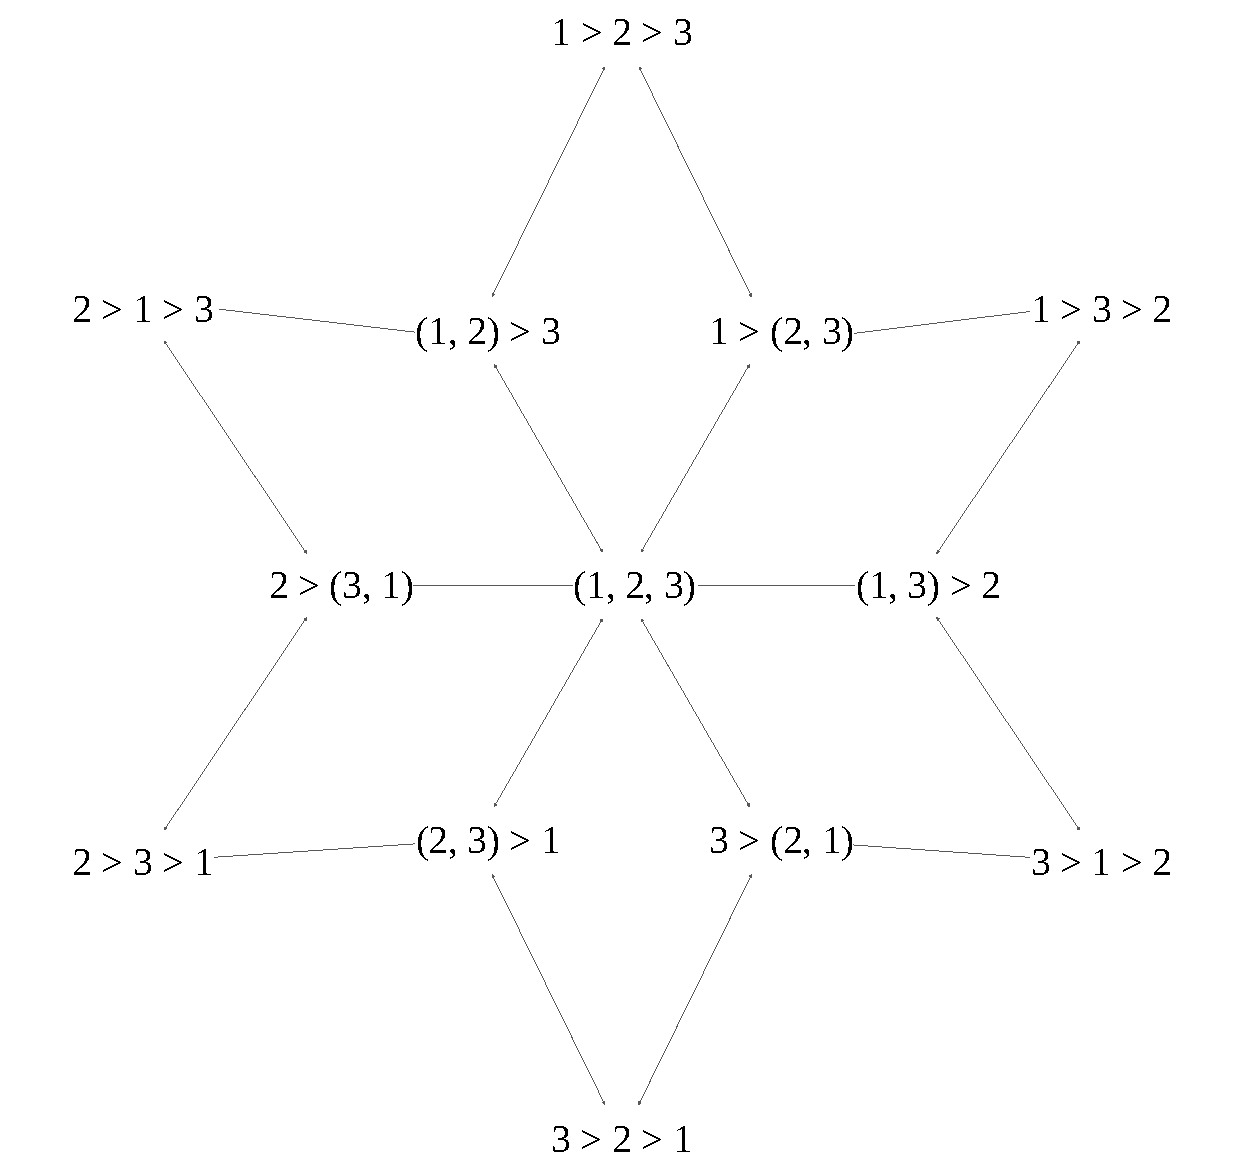
\includegraphics[width=0.65\textwidth]{dpGraph.pdf}
    \caption{The graph of judgement sets for all preferences over three alternatives.}
    \label{figure:DPDistance}
\end{figure}

Apart from there distances, they also define a voter as a tuple of a (weak) preference and a bias (towards their current position) \(v = \langle r, b \rangle \), with \( b \in \Reals_{[0,1]}\). Finally, a deliberation step \(D_{s} : V \times r \mapsto V\), with $V$ being a set of voters and $s$ being one of the spaces (KS, DP, CS). A round of deliberation consists of $n$ deliberation steps, where each voter has announced their opinion once. We formulate this procedure in the following program:
\IncMargin{1em}
\begin{algorithm}
    \SetKwInOut{Input}{input}
    \SetKwInOut{Output}{output}

    \Input{Set of Voters $V$, metric space $s$}
    \Output{Updated set of Voters $V$}
    \BlankLine

    $V_{\text{u}} \gets V$ \tcp*[h]{Set of unannounced voters (references to $V$)}\\

    \While{$|V_{\text{u}}| > 0$}{
    Select a random $v \in V_{\text{u}}$\\
    $V_{\text{u}} \gets V_{\text{u}} \setminus \{v\}$\\
    $V \gets D_s(V, v.r)$ \tcp*[h]{Update voters based on $v$'s preference}
    }

\end{algorithm}
\DecMargin{1em}

The deliberation step $D_s$ then updates all voters such that their new preference  minimizes the following formula.
\begin{equation}
    r =
    \sqrt{
        b d_s(r_i, r')^2 + (1-b)d_s(r_j, r')^2
    }
    \label{eq:deliberation_step_formula}
\end{equation}
Where $r_i, r_j$ are the voters and the announced preference, respectively, and $r'$ is the voters new preference.

We present a replication and extension of their work \cref{experiment_results}. Furthermore, we present novel results based on this model in \cref{theory}.

 %Related literature and material (8-12 pages)
\chapter{Methods}
\label{Methods}
\lhead{\emph{Methods}} % Set the left side page header to "Symbols"

We proceed with the methods used to replicate the paper by
\citet{radDeliberationSinglePeakednessCoherent2021}, as well as the
experimental setup of our own model. Links to the data used for these
experiments can be found in \Cref{ethics_data}. The programs
are implemented using \texttt{OCaml}, and \texttt{Python}.


\section{Replication} We implement the model as described in
\Cref{section:related_work}. Agents are limited to strict preferences over all
candidates. All experiments are done with 3 alternatives, and 51 voters. The
number of voters is chosen to be an odd number, as this prevents ties between
alternatives. We measure evaluations relating to strict preferences, namely the
proportion of cyclic Profiles, the Number of Unique profiles and the proximity
to single-peakedness by voter deletion (PtS-V), as reported by
\citet{radDeliberationSinglePeakednessCoherent2021}. In addition to those we
also measure the number of Condorcet winners. We do not measure the PtS-C, as
any profile with 2 candidates is single-peaked, thus given the simulation will have 3 candidates
this metric would be of little added value, as all values would be either 1 or $\frac{2}{3}$.

\section{Experiments}

We aim to replicate the findings by the \textsc{America in One room}
experiments \cite{fishkinCanDeliberationHave2024} in-silico. To this end we
use the adaption to the DeGroot model as laid out in \Cref{sec: main model}
The dataset contains a control group as well as an experimental group. In the
dataset, the control group shows no change in opinion over time,
thus this group is best modelled by using the identity matrix $I^n$ as the
trust matrix. The experimental group is modelled as a densely connected
network.  The distribution of the trust we control through 3 methods.

\subsection{Modelling Trust} We propose three different mechanisms through which we
will the trust matrix, as well as the intuitive and theoretical
appeal.

% \textbf{Connectedness}. Firstly, a decision has to be made on whether
% voters in the model are able to communicate with all other voters, if this is the case, we
% get a strongly connected graph, otherwise some voters might not share an edge.
% In the case of small scale deliberation, one might reasonably argue that, at
% least in principle, voters should be able to listen to all other participants,
% and use these opinions to inform their own. In larger settings, such as social
% media platforms or large gathering, it seems that a person's ability
% to communicate effectively with everyone diminishes as the group size grows. In this work, we take
% this to be the main characterization ``true'' deliberation, namely the ability
% to listen to all other participants.

\textbf{Knowledge}. Firstly we consider knowledge, this can be used to
inform both the trust in others, and your bias towards yourself. For this we
can imagine a vector $\boldsymbol{k}$, where each $k_i$ contains some knowledge
score for voter $i$. In modeling, we now have 2 options, firstly, does a voters
knowledge affect their bias towards their own opinion. Intuitively one could
reasonably argue either way. Two plausible ways of reasoning are, ``A
knowledgeable voter knows more facts and is therefore harder to convince'', or
``A Knowledgeable voter realizes the complexity of the topic and is therefore
less certain''. The first line of reasoning seems more general, as it seems
independent of the topic at hand. However, the second line of reasoning seems
to capture something like the Dunning-Kruger effect, which states that people
can have ``meta-ignorance'', meaning they do not realize what they do not realize.

As for the trust a voter places in their peers, a similar argument can be made,
where the voter could either place more trust on people that are more
knowledgeable, and thereby might be able to provide more facts. Or they could
trust less knowledgeable people more because their ignorance allows them to
make more confidant claims, even if these are inaccurate.


\textbf{Similarity}. Finally, voters might simply trust people with
similar opinions more, representing a sort of confirmation bias. This cannot be
applied to ones own opinion in the same sense as with the other two methods.
This could be represented as a sort of ``general bias'', where a voter is more
or less inclined to listen to other opinions.

\textbf{Ego}. Lorem Ipsum.

Given these different options, the right selection of methods becomes question
for empirical observation, which we present in the next Chapter.

Firstly, and most simply, we give all voters a bias. This bias reflects how
much of their trust they place on themselves. For example a bias of 1
represents them placing equal trust on themselves as all other voters combined.
The actual weight on the self loop is calculated as the sum of all incoming
edges multiplied by the bias. Secondly, we have knowledge-based trust, in which
a voter trusts voter $j$ more if voter $j$ is more knowledgeable. We get the
knowledge scores from the \textsc{America in One room} dataset by taking the
proportion of knowledge questions they answered correctly. The interpretation
is that more knowledgeable voters would be more persuasive and thus be more
influential on other voters' opinions. Thirdly, we have credibility-based
trust, where the trust a voter places on another voter is proportional to the
number of outgoing edges that second voter has. This method becomes equivalent
to placing uniform trust in all voters when all voters are situated in a fully
connected graph. If we do not use credibility- or knowledge- based trust, we
call this uniform trust, meaning that they treat all neighbors the same.
Importantly, this does not imply any specific bias value.



\subsection{DeGroot extension}

The first experiments we perform concern the DeGroot model. These experiments
consist of two parts. Firstly we search the parameter space to identify
parameters that best replicate the data, using Bayesian Parameter Estimation.
For this we use data from the \textsc{America in One room} experiment as
described in \Cref{section:related_work}. Though this data does not provide
full preference rankings over the candidates, it does provide data on voters'
opinions on 6 different topics of political discussion, such as climate change
and immigration. Using these opinions, we are able to generate potential
candidates, this is done either by selecting a voter and creating a candidate
with identical opinions, or by pooling 10 voters\footnote{This is arbitrary,
	and it might be good to look into this, but in my opinion this is low priority
	for now. It might also be useful to keep the candidates constant over the
	course of an experiment}
and creating an average of their opinions. Using these
simulated candidates we are able to create preference rankings using the
$\ell_1$-norm. To model the difference between the deliberation and control
group we change the topology of the graphs voters in the respective groups are
situated in. As mentioned before, the deliberation groups will be embedded in a fully connected
graph, while the control groups will be placed on the graph of academic
citations in physics \cite{nr}, this graph is small enough to
allow sampling of the graph for each simulation. Since the original data
provides group numbers for candidates who participated in the deliberation, we
also experiment with replicating these groups as opposed to randomly grouping
voters together.


We measure whether the final profiles are cyclic, whether they have a Condorcet
winner, home many unique profiles there are, and their proximity to being
single-peaked. Proximity to single-peakedness is measured in two ways. When the
simulation size allows for it, we measure the proximity in terms of the number
of voters that would need to be removed for the full profile to become
single-peaked. This particular notion is NP-complete
\cite{erdelyiComputationalAspectsNearly2013}, though it allows for a
2-approximation. We use the method based on an ILP solver, as implemented in
\texttt{PrefTools} \cite{PrefLibPreflibtools2025}. The other notion of proximity is the proximity in
terms of the number of candidates that need to be removed for the profile to
become single-peaked. This can be done in $\mathcal{O}(|V| \cdot{} |C|
	^3)$\cite{przedmojskiAlgorithmsExperimentsNearly}, though the implementation we
use is that of the \texttt{PrefTools} library \cite{PrefLibPreflibtools2025}, which implements
a slower $\mathcal{O}(|V| \cdot{} |C|^5)$ algorithm
\cite{erdelyiComputationalAspectsNearly2013}.




% We aim to find values for all parameters that minimize the error of the model,
% conditional on the number of voters and candidates. For this we define the
% error of our model as the (normalized) difference of the proportion of cyclic
% profiles, the proportion of simulation containing a Condorcet winner, and the
% proximity to single-peakedness through voter deletion, and the
% candidate-based notion. With these parameters, we argue that model captures the
% learning process. We then proceed to analyze convergence behavior under these
% optimal parameters. For this analysis, all configurations are run 100 times.


\renewcommand{\arraystretch}{1.2}
\begin{table}
	\centering
	\begin{tabular}{p{4cm}p{0.65\linewidth }}
		\toprule
		Parameter                     & Description                                                                                                                                      \\
		\midrule
		\texttt{Number of Voters}     & The number of voters in the simulation, representing either the deliberation group, or the control population.                                   \\
		\texttt{Number of Candidates} & The number of candidates to be voted on.                                                                                                         \\
		\texttt{Candidate Generator}  & The way the candidates are generated. Either a random voter is selected for each candidate, or 10 random voters (sampled with replacement) get averaged into one candidate. \\
		\texttt{Bias}                 & The bias all voters have towards their own opinion.                                                                                              \\
		\texttt{Time steps}           & The number of deliberation ``steps'' the voters undergo.                                                                                         \\
		\texttt{Group}                & Use the original groups.                                                                                                                         \\
		\texttt{Similarity}           & Distribute trust based on credibility.                                                                                                           \\
		\texttt{Knowledge}            & Distribute trust based on knowledge.                                                                                                             \\
		\texttt{Ego}                  & Scale voters' bias according to the trust other people have in them                                                                              \\
		\texttt{Self-Knowledge}       & Scale voters' bias according to their knowledge                                                                                                  \\
		\bottomrule
	\end{tabular}
	\caption{The parameters of the DeGroot learning based model, as well as their descriptions}
\end{table}

Given the best configurations, we will analyze the behavior of the model to
understand the convergence on opinion. To this end, we measure the change in the trust
matrix, as well as the distance between each voter's pre- and post-deliberation
preferences using the KS and CS distances. We first aim to find the number of
deliberative steps needed for convergence, which we define as the moment where
the largest change in the trust matrix is smaller than some $\epsilon$. Then we
hope to understand how individual voters' opinions change by looking at the
final state of the trust matrix.

Finally, we use sensitivity analysis to investigate which parameters have the
strongest effect on the model, using Sobol indices to get the first and second
order effects.

 %Details of your approach (10-15 pages)
\newpage
\chapter{Experimental Results}
\label{experiment_results}
\lhead{\emph{Experimental Results}}
We first present a full replication and extension of the work by
\citet{radDeliberationSinglePeakednessCoherent2021}. Then we present the
simulations based on our model of meta-deliberation, as well as the results of
the sensitivity analysis on both models. All code for the replication, main
experiment and visualizations can be found in
\href{https://github.com/amirsahrani/master_thesis}{this Repository}.


\section{Replication} We are able to fully replicate the results found by
\citet{radDeliberationSinglePeakednessCoherent2021},  in \Cref{fig:rep_cyclic}
we see that while the bias is less than 0.73, all metric results in a-cyclic
preferences. We also replicate the behavior of the KS metric, where biases in
the range of 0.73-0.85, show even some initial a-cyclic profiles can become
cyclic. \Cref{fig:rep_count} Further explains this by showing that within this
range we always observe 3 unique profile for the KS metric, while DP and CS
have already settled on 6 profiles, thereby representing all possible
preferences. \Cref{fig:rep_condorcet} shows KS introduces ambiguity in the case
that there was a Condorcet winner, resulting in losing the original nice
profile. Finally, the proximity to single-peakedness shows a slightly more
positive note for the KS metric, showing that while the DP and CS bottom out to
the minimum proximity to single-peakedness, KS stays relatively close. Though
this should be taken with a grain of salt, as it is likely a consequence of the
unique preferences being smaller.

\begin{figure}[htbp]
	\centering
	\begin{minipage}{0.45\textwidth}
		\centering
		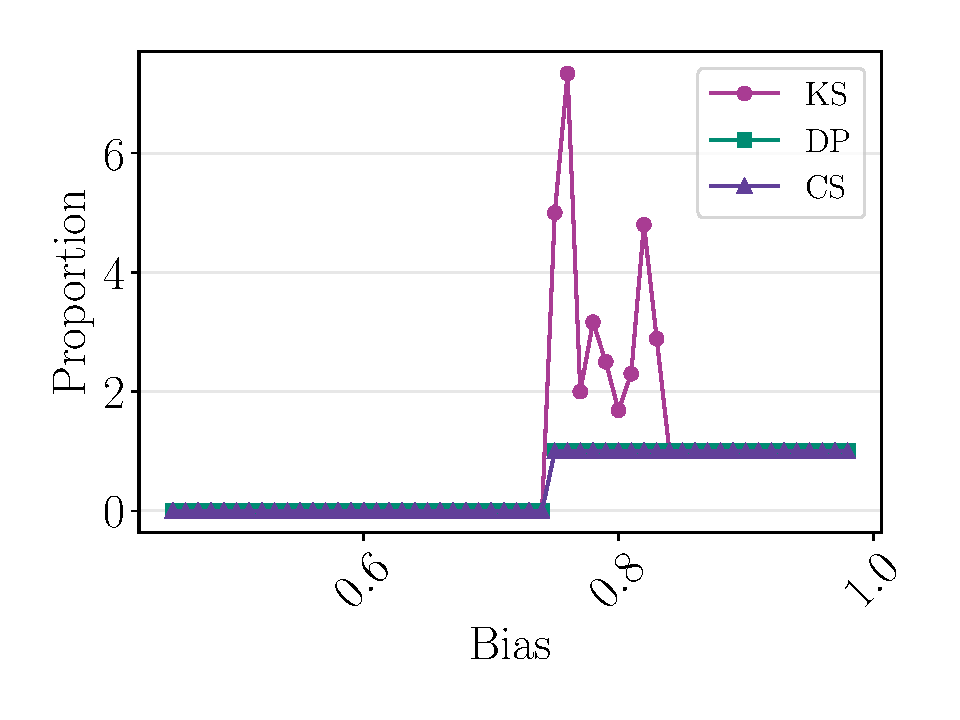
\includegraphics[width=\textwidth]{Figures/cyclic_proportion_Proportion.pdf}
		\caption{The proportion of cyclic profiles remaining, 0 indicating that no cyclic profiles were present after deliberation.}
		\label{fig:rep_cyclic}
	\end{minipage}\hfill
	\begin{minipage}{0.45\textwidth}
		\centering
		\vspace{-9pt}
		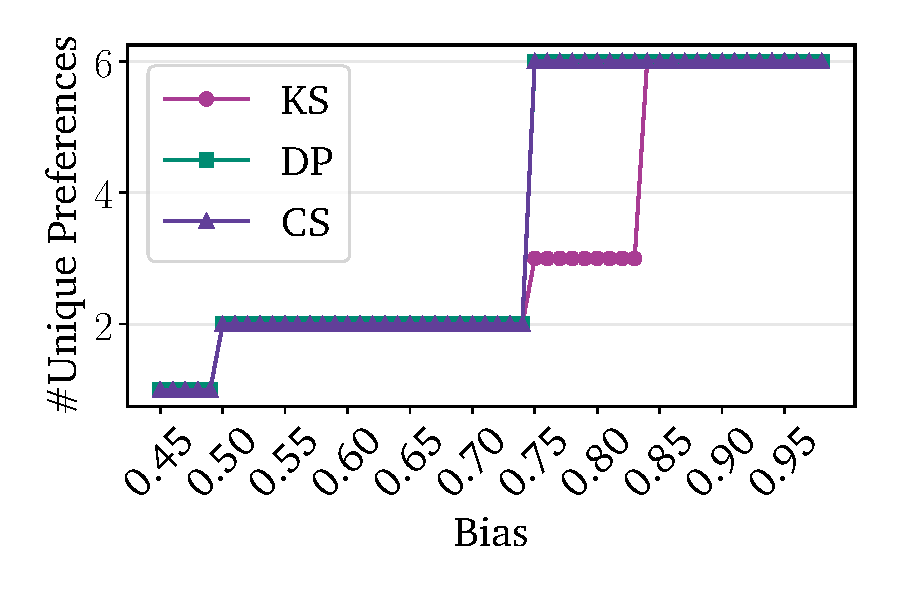
\includegraphics[width=\textwidth]{Figures/unique_Unique Preferences.pdf}
		\caption{Number of unique preferences at the final step of deliberation.}
		\label{fig:rep_count}
	\end{minipage}

	\vspace{1em}

	\begin{minipage}{0.45\textwidth}
		\centering
		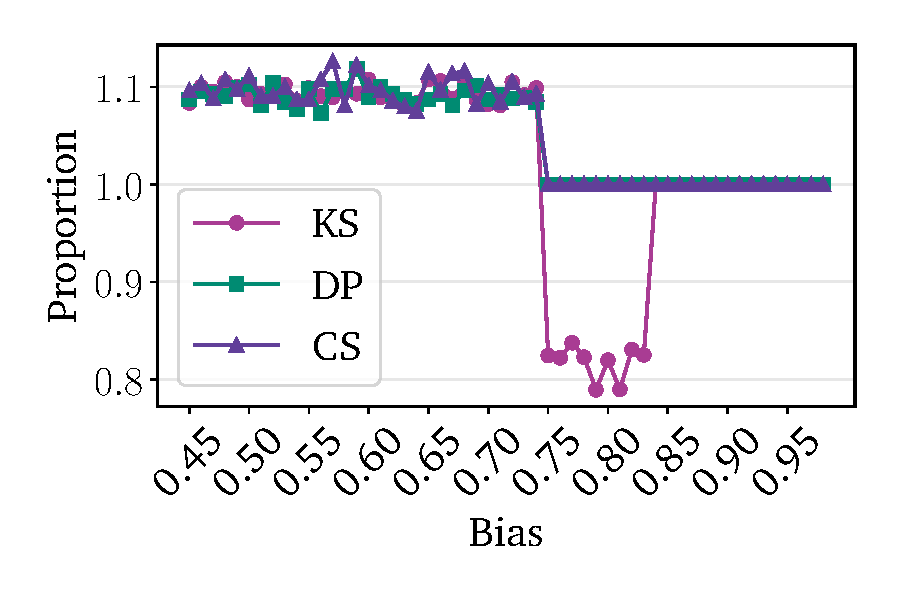
\includegraphics[width=\textwidth]{Figures/condorcet_proportion_Proportion.pdf}
		\caption{The proportion of Condorcet winners left after deliberation, value above one indicate Condorcet winners emerging during deliberation}
		\label{fig:rep_condorcet}
	\end{minipage}\hfill
	\begin{minipage}{0.45\textwidth}
		\centering
		\vspace{-9pt}
		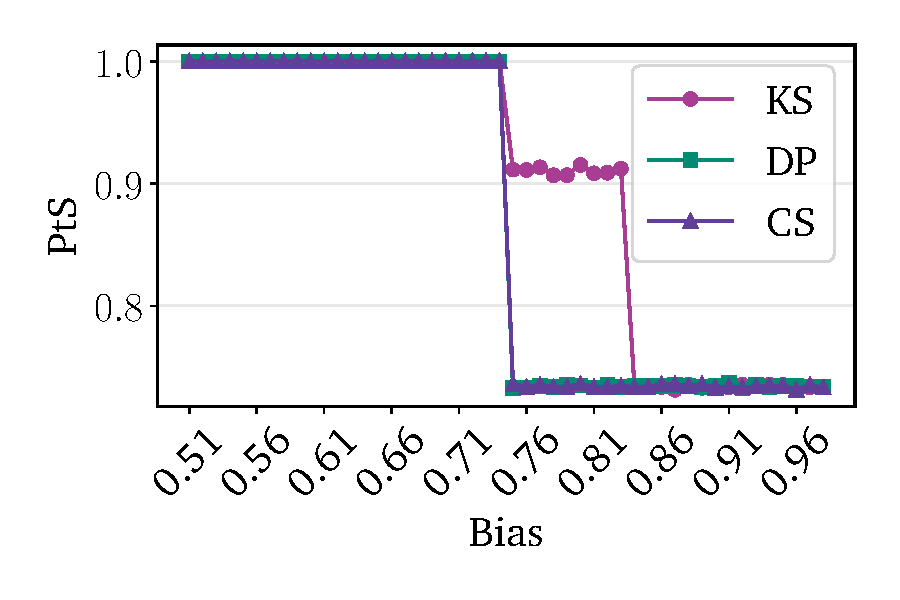
\includegraphics[width=\textwidth]{Figures/sp_proximity_PtS.pdf}
		\caption{Proximity to single-peakedness after deliberation. Proximity to single-peakedness as defined in \Cref{section:related_work}.}
		\label{fig:rep_single_peaked}
	\end{minipage}
\end{figure}

\newpage
\section{DeGroot Model}
\label{degroot_results}

We now present the results of our model based on the DeGroot learning process.
The deliberation group, which is supposed to represent a small group with
deeper talks with everyone on the group, is analysed first. The deliberation
group is modelled as a dense graph, with a few voters. Though the original data
supplied group numbers, for these experiments voters were assigned to their
groups arbitrarily. In terms of the final measures, we focus on whether the
final profiles are cyclic, whether they have a Condorcet winner, home many
unique profiles there are, and their proximity to being singly peaked.
Proximity to single peakedness is measured in two ways. When the simulation
size allows for it, we measure the proximity in terms of the number of voters
that would need to be removed for the full profile to become singly peaked.
This particular method is NP-complete
\cite{erdelyiComputationalAspectsNearly2013}, though it allows for a
2-approximation, we cannot reliably use it for larger groups, given the
sheer number of simulation necessary. The other notion of proximity, which we
will always measure, is the proximity in terms of the number of candidates that
need to be removed for the profile to become singly peaked. This can be done in
$\mathcal{O}(|V| \cdot{} |C| ^3)$\cite{przedmojskiAlgorithmsExperimentsNearly}, though the implementation used is
that of the \texttt{PrefTools} library \cite{preftool}, which implements a slower
$\mathcal{O}(|V| \cdot{} |C|^5)$ algorithm
\cite{erdelyiComputationalAspectsNearly2013}. 



\renewcommand{\arraystretch}{1.2}
\begin{table}
	\centering
	\begin{tabular}{p{4cm}p{0.65\linewidth }}
		\toprule
		Parameter & Description  \\
		\midrule
	\texttt{Number of Voters} & The number of voters in the simulation, representing either the deliberation group, or the control population.\\
	\texttt{Number of Candidates}  & The number of candidates to be voted on. \\
	\texttt{Candidate Generator} & The way the candidates are generated. Either a random voter is selected for each candidate, or 10 random voters get averaged into one candidate.\\
	\texttt{Bias}& The bias all voters have towards their own opinion. \\
	\texttt{Time steps}& The number of deliberation ``steps" the voters undergo.\\
		\bottomrule
	\end{tabular}
	\caption{The parameters of the DeGroot learning based model, as well as their descriptions}
\end{table}

We use the \textsc{America in One room} dataset
\cite{fishkinCanDeliberationHave2024} for the support vectors of all
voters. As this dataset does not contain full preference rankings, we validate
the explanatory power of the model as follows. We aim to show that under
different numbers of voters and candidates and different ways to generate
candidates, we can find bias factors and deliberation times which minimize the
error of our model. Through showing these positive results for multiple
different (plausible) scenarios we argue that model does capture the learning
process. We then proceed to analyse the results in relation to this dataset,
interpreting the optimal bias values, as well as looking at the rate of
converges given "optimal" parameters. For this analysis, all configurations
were run 100 times.


\subsection{Optimal parameters}

Between the deliberation group and the control group, if we look at the final
time step, we find that both perform best if the bias is set to be around 1,
though this differs based on the other parameters. This seems to indicate that
for both smaller and larger groups, a voter's opinion is in some sense equally
important as the of  \textit{all} other voters she comes in contact with. In
other words, it does not seem to matter how many people disagree with a voter,
her own opinion holds a constant relative importance.

Looking at the deliberation group, we show the best bias values in the following table:
\begin{table}[ht]
\centering
\begin{tabular}{ccccccc}
\toprule
$n_\text{candidates}$ & $n_\text{voters}$ & MSE (Sample) & MSE (Voter) & Bias (Sample) & Bias (Voter) \\
\midrule
3 & 9  & 0.00747 & 0.00733 & 1.3 & 1.3 \\
3 & 11 & 0.00951 & 0.00969 & 1.2 & 1.0 \\
3 & 13 & 0.00978 & 0.01080 & 1.2 & 1.2 \\
3 & 15 & 0.01409 & 0.01231 & 1.3 & 0.9 \\
5 & 9  & 0.03244 & 0.05191 & 0.8 & 1.1 \\
5 & 11 & 0.05640 & 0.05591 & 1.4 & 0.9 \\
5 & 13 & 0.07609 & 0.08720 & 1.1 & 0.8 \\
5 & 15 & 0.06716 & 0.07476 & 0.9 & 0.9 \\
7 & 9  & 0.07412 & 0.18686 & 1.3 & 1.2 \\
7 & 11 & 0.12538 & 0.17129 & 1.2 & 1.3 \\
\bottomrule
\end{tabular}
\caption{Minimum mean values at time step 151 for each candidate selection method, with corresponding bias.}
\label{tab:min_mean_bias_delib}
\end{table}

Here it is clear that generally the model performs best when both the number of
candidates and the number of voters are low. We also not that though the error
of the different candidate generators are comparable, they in general the
Sample methods seems to results in larger errors, meaning that the model is
less well able to capture circumstances where the alternative's opinions are
not represented in the deliberating population. Finally, we see that The
distribution of best biases skews to values around 1.3, thus indicating that
even while deliberating, people tend to hold their opinion to be \textit{more}
important than that of all other voters.

We investigate this discrepancy between the two candidates generation methods
now, to this end we look at the difference in error for all tested
configuration. 

% Now we T test on everything the Sample and Voter method

\subsection{Convergence}

From \Cref{theory}, we have seen that in the limit some matrices are
convergent, while some are not, in particular if the matrix is aperiodic, this
it is convergent. For the matrices in these simulations, we cannot guarantee 
aperiodicity. Thus, we resort to the following, instead of looking at the
matrices directly, we instead look at the distance between the estimated
support matrix, and the true support matrix, where the distance in the element
wise $\ell_2$ norm. We do the same for the support vectors and the true
opinions.

....


We find ....


\subsection{Single-peaked Preferences}

We now proceed to look at distance to single peaked profiles, look at both
voter removal and candidate removal. We show that for optimal bias, as
deliberation progresses we see an increase in the proximity to single
peakedness.

...
 %Evaluation/testing of your hypothesis (10-15 pages)
\newpage
\chapter{Discussion}
\label{Discussion}
\lhead{\emph{Discussion}}


% Methodological Limitations
% Trust matrix generation mechanisms, e.g. race voice etc.
% Uniform trust between substantative and meta
% 

% Broader implications

% If the Degroot model is accurate, more deliberation would lead to
% substantative agreement, this however is undermind by fishkins "Can
% deliberation have lasting effects", because at least in practice this was
% long and intense, therefore in general it is unreasonable to expect to have
% voters deliberate even longer. 

% This model aligns with that the idea that deliberation pulls extreme opinions
% to middle, such as those from psychology about in-group out-group opinion
% change. There it is established that if groups have little contact they
% become more different
% as each group becomes more alike with-in the group, therefore pull the means of
% the two polarized groups away from each other

% DeGroot model is an insufficient heuristic to model the type of "learning" done
% during deliberation

% Formal model likely unable to fully capture intricacies of interpersonal interaction
% that occurs during deliberation. This is to say, the model might not have predicted
% the change in opinion accurately, but nevertheless we can still learn from this and note
% that deliberation has more complex interactions than a simple weighted linear average.





\section{Conclusion}

We have shown deliberation to be susceptible to strategic manipulation under
various notions of strategic manipulation. Most importantly, we have defined a
new notion of strategyproofness specifically for deliberation over preference
profiles. As a result, we caution that even when deliberation succeeds in
producing single-peaked profiles, it does not guarantee fairness. In the sense
that if all voters had been honest during deliberation, the resulting profile
might have differed. Intuitively, this is expected, as individuals may pretend
to hold more extreme views to shift the general consensus.

Given the idea that  deliberation encompasses more than preferences alone, we
extended our model to deliberation over opinions of voters and alternatives,
through an adaptation of the DeGroot model. We also demonstrated that finding a
voter graph that minimizes the difference between opinion distance and graph
distance is NP-Hard. Suggesting that, in practice, modeling voters on sparse
graphs requires collecting both communication patterns and opinion data. 

Though we were able to replicate the results be
\citet{radDeliberationSinglePeakednessCoherent2021}, we note that the model is
too restrictive, as it only concerns itself with full preferences. We find that
for certain ranges of bias the model behaves chaotically, and introduces cyclic
profiles, even if before the deliberation these were acylic for the KS distance
measure. Given that this model strictly models preferences, we extend it to a 
DeGroot learning model to incorporate opinions in general.

The DeGroot model successfully predicts opinion shifts at the population level
but performs poorly at the level of individual voters. Extending the
simulations to include deliberation on candidate positions, that is, on
meta-opinions, yields profiles with more similar characteristics to the true
preferences. However, after a few iterations, preferences converge too
strongly, resulting in profiles that are less cyclic and more single-peaked
than reality. We note that the development of proximity to single-peakedness
(for both candidate and voter deletion) follows a sigmoid curve, characterized
by a gradual start, a phase of rapid change, and eventual convergence.

Our sensitivity analysis shows that all model parameters influence outcomes.
However, only parameters tied to knowledge and voter count exert strong direct
effects — likely because they introduce new information, whereas other
parameters only modulate existing dynamics. In terms of predicting final PBS,
we found that Ego-based bias and knowledge-based trust performed best. Thereby
indicating that more knowledgeable people are more convincing in deliberation,
while people become less likely to change their minds if many people value
their opinion. This is an intuitive result, but as mentioned
\Cref{experiment_results}, we caution that the reason for Ego-based bias
performing well might be (partly) explain by simply reducing the change in
opinions of voters.

In general political elections might elect candidates that will bring about
many changes, most voters however will not have a strong opinion on all of
these. Though we investigated the change in opinion on a per-topic basis, 
we were unable to incorporate this in the preferences over candidates. Given
that most change in opinion was on immigration and healthcare, it might be
the case that these topics were considered more important for this election
and thus more time was spent discussing these. As a result the preferences 
of voters over candidates might be influence more strongly be these topics. 

% - Explain general implications of these results
% 	- Link back to core principles of Deliberation (Honesty etc.)
% 	- Explain how in real life honesty can be safe guarded?
% 	- Put in context of deliberation interventions



\section{Limitations}

\subsection{Applicability of results}
% Practical matters, irrespective of what the model does and does not take into account

While the DeGroot model has been shown to be a more accurate representation of
human belief updating than full Bayesian updating, it does not take into
account why people hold certain beliefs, not does it constraint what kinds of
beliefs a voter can hold at the same time. To remedy this, one might consider a
framework such as abstract argumentation theory (source (DUNG 1995)), as this
is able to model the arguments with the deliberative groups. Though, this seem
theoretically nice, as it allows for formal description on why opinions and
preferences are held, not just descriptions of these facts. From a simulation
based perspective, such a model introduces major validity question. Firstly the
framework requires a map on the relation of all arguments, for this one does
not only need qualitative data, i.e. reported arguments by participants, but
also a method of reliably and accurately transforming these qualitative reports
to argumentative graphs. Secondly, the abstract argumentation framework does
not pose an updating mechanism, thus the method through which participants
would updates their believes using this framework is unclear.

The choice of the DeGroot model assumes that people linearly interpolate between
opinions presented to them. While it has been shown that in some circumstances 
this is a good heuristic, especially when compared to full Bayesian updating. It
does limit the behavior of voters substantially.  
% Now merge into this the section
% on how voters can have contradictory opinions in this model. Also mention mention
% voters might not actually linearly move. An example could be voters having a "threshold"
% for when they would change their mind.

Furthermore, our negative results on strategic manipulation might be remedied
in human deliberation. As fellow participants might be able to sense that
someone is being dishonest. It is also not unreasonable to think that someone
pretending to hold a different opinion, might be worse at defending this
opinion, and therefore be less persuasive.

In the testing of our model, we have consulted a single dataset containing a
large amount of information need. 
However, as a result of not having a single
data set which can fully inform the values in our model, multiple strong
assumptions have been made in order to test the feasibility of the model. We
mention these explicitly once more, as well as how what kind of data might be
collected to inform this and similar models. We formulate this in terms of
missing information on voters and candidates respectively, and present some of
the most important limitations of each.


\subsection{Voter information}
% Issues relating to information we have on the voters

Firstly, we have no access to a data set containing opinions before and after
deliberation as well as the corresponding preference orders. This means having to infer
preferences over candidates, though we chose to do this by minimizing the
distance between the voter and the alternatives, reasonable alternatives exist.
For example, people might use different heuristics to locate a few alternatives
they like best, such as ``Agrees with me on important topics'', thus putting weight on certain issue dimensions. Or they might
simplify each comparison to "Agrees or Disagrees" with me, with some range of
opinion they consider to be in agreement with theirs. 

Furthermore, the way we encode voters' information on alternatives might not
accurately reflect true voters' information. One might expect voters to be more
familiar with candidates close to them in opinion, and thus have less noisy
estimates of these candidates' positions. 

Finally,  the error of voters' estimates might not be normally distributed. In
a polarized election, it is not unreasonable to expect errors on the
``opposing'' party to skew further way from that voters' opinion.


\subsection{Candidates}
% Issues we have realting to information we have on candidates (which is effectively no information)

Though datasets such as those by Ipsos might contain the scores of political
parties, these datasets cannot (easily) be combined with the data used in this
study. This is mostly due to the inconsistent formats of the questions and the
included topics. As a result, we are required to generate candidates manually.
Thereby not only introducing another modeling choice, but also discarding an
important piece of information. The \textsc{America in One Room} dataset does
contain voters' most preferred candidate, which is either the Democratic or
Republican Party or Independent (participants are not asked to further
specify). But lacking information on the candidates true positions as well as
the ranking over the others, this information is hard to incorporate within the
model. 

Instead, we chose a simple approach, either selecting a single
voter, or grouping some voters together as a single candidate. In the real
world, however, candidates might arise in different ways and forms. For
example, they could bring new idea's, not measured in the poll, or gather
like-minded people instead of catering to the entire voting population, indeed
the latter seems to be point of representative democracies. In representative
democracies candidates represent specific demographics of the population, and
advocate for their interests.


\subsection{Extentions}
% First extend model in terms of deliberation, then possibly as a model of population


Given the weak performance of the model, a better computational model is needed
to understand deliberation and inform the design of deliberative interventions.
We propose some extensions to the model, which might better capture human
dynamics.

When humans deliberate, the amount of trust placed on each person is likely not
fixed, for example, if someone has convinced a voter to change their mind on
multiple topics, this voter might be more likely to trust them on a new topic
as well. Or on the contrary, if two voters consistently disagree, and diverge
in their opinions, they might come to trust each other less. Furthermore, the
development of trust will likely differ between people, both on their baseline
and development of their trust. Though we do not propose a specific updating
scheme for this, the model is flexible enough to allow for the updating of the
trust matrix over time. 


If we extend this model to model large population, for example using a social
network, it is crucial to be able to assess the effects disruptive events such
as a national health crisis, an economic recession or a national safety threat.

As a result of such an event subset of the voters might become more informed on the position of
the candidates, as the event might cause information dispersal, for example
through news networks. This limitation is related to the notion of
\textit{Salience} as described by
\citet{listDeliberationSinglePeakednessPossibility2013}, stating that topics
with high salience benefit less from deliberation, as participants have likely
received more information on this topic. Though this could, at least in
principle, be resolved by constructing trust matrices for individual topics.
This would raise further questions as to the validity of these matrices.
 %Evaluation/testing of your hypothesis (5-8 pages)
\input{Chapters/ConclusionsandFutureWork} % (5-6 pages)
\newpage
\chapter{Ethics and Data Management}
\label{edm}
\lhead{\emp{Ethics and Data Management}}
A new requirement for the thesis is that there must be a short section in which you reflect on the ethical aspects of your project. This requirement is related to one of the final objectives that a graduated student of the Master of Computational Science must meet: “The graduate of the program has insight into the social significance of Computational Science and the responsibilities of experts in this field within science and in society". You don't need to devote an entire chapter to this; a short section or paragraph is sufficient.

I acknowledge that the thesis adheres to the ethical code (\url{https://student.uva.nl/en/topics/ethics-in-research}) and research data management policies (\url{https://rdm.uva.nl/en}) of UvA and IvI.

The following table lists the data used in this thesis (including source codes). I confirm that the list is complete and the listed data are sufficient to reproduce the results of the thesis. If a prohibitive non-disclosure agreement is in effect at the time of submission ``NDA" is written under ``Availability" and ``License" for the concerned data items.

\begin{table}[h]
	\centering
	\begin{tabular}{lll}
		\textbf{\begin{tabular}[c]{@{}l@{}}Short description \\    (max. 10 words)\end{tabular}} & \textbf{\begin{tabular}[c]{@{}l@{}}Availability \\    (e.g., URL, DOI)\end{tabular}} & \textbf{\begin{tabular}[c]{@{}l@{}}License \\    (e.g., MIT, GPL, CC)\end{tabular}} \\ \hline
		Example dataset 1                                                                        & \textless{}github url\textgreater   or Figshare                                      & GPL                                                                                 \\ \hline
		Example source code                                                                      & DOI (from Zenodo)                                                                    & MIT                                                                                 \\ \hline
		Example sensitive   data                                                                 & NDA                                                                                  & NDA                                                                                 \\ \hline
	\end{tabular}
\end{table}


%----------------------------------------------------------------------------------------
%	THESIS CONTENT - APPENDICES
%----------------------------------------------------------------------------------------

%\addtocontents{toc}{\vspace{2em}} % Add a gap in the Contents, for aesthetics

%\appendix % Cue to tell LaTeX that the following 'chapters' are Appendices

% Include the appendices of the thesis as separate files from the Appendices folder
% Uncomment the lines as you write the Appendices

%% Appendix A

\chapter{Extended Proofs}

\label{AppendixA} % For referencing this appendix elsewhere, use \ref{AppendixA}

Finally, for \textit{CS}, $R_{1}$ and $R_{j}$ stay the same, while $R_{1}^{'} = c \pref a \pref b \pref \cdots \pref m$, resulting in $\operatorname{Dist}_{\text{CS}}(R_{1}^{'}, R_{j}) = |2-2| + |1-3| + |3-1| = 4$.


%% Appendix A

\chapter{Extended Proofs}

\label{AppendixA} % For referencing this appendix elsewhere, use \ref{AppendixA}

Finally, for \emph{CS}, $R_{1}$ and $R_{j}$ stay the same, while $R_{1}^{'} = c \pref a \pref b \pref \cdots \pref m$, resulting in $\operatorname{Dist}_{\text{CS}}(R_{1}^{'}, R_{j}) = |2-2| + |1-3| + |3-1| = 4$.


%\input{Appendices/AppendixC}

\addtocontents{toc}{\vspace{2em}} % Add a gap in the Contents, for aesthetics

\backmatter

%----------------------------------------------------------------------------------------
%	BIBLIOGRAPHY
%----------------------------------------------------------------------------------------

\label{References}

\lhead{\emph{References}} % Change the page header to say "Bibliography"

\bibliographystyle{unsrtnat} % Use the "unsrtnat" BibTeX style for formatting the Bibliography

\bibliography{references}

\end{document}  
